\documentclass{beamer}

\usepackage[utf8]{inputenc}
\usepackage[T1]{fontenc}
\usepackage[french]{babel}
\usepackage[ddmmyyyy]{datetime}

\usetheme{Warsaw}
\useinnertheme{rectangles}
\setbeamerfont{headline}{size=\large}
\setbeamerfont{frametitle}{size=\normalsize}

%Plan/Sommaire automatique avant chaque section
\AtBeginSection[]{
  \begin{frame}
  \frametitle{Plan}
  \tableofcontents[currentsection]
  \end{frame}
}

\author{Sonny Klotz - Jean-Didier Pailleux - Malek Zemni}
\institute{UVSQ}
\date{\today}
\usepackage{../tex/myInfolines}
\usepackage{longtable,array}
\title{Présentation Cahier des Charges}

\begin{document}

	\begin{frame}
		\titlepage
	\end{frame}
	
	\section{Introduction}
	\begin{frame}
		Projet de L3 informatique UVSQ, remis par DCbrain.\\~\\
		Le travail est décrit dans ce cahier des charges :
		\begin{itemize}
			\item Motivations
			\item Contraintes
			\item Exigences fonctionnelles
			\item Exigences non fonctionnelles
			\item Autres aspects du projet
		\end{itemize}
	\end{frame}
	
	\section{Motivations du projet}
	\begin{frame}
		\textbf{Problème :} masses de données importantes et difficilement exploitables
		\textbf{Objectif :} fournir un outil d'analyses préliminaires de ces données
		\\~\\
		\pause
		\textbf{Parties prenantes :} \pause
		\begin{itemize}
			\item \textbf{Maitre d'ouvrage :} DCbrain, module Projet de l'UVSQ
			\item \textbf{Client :} DCbrain
			\item \textbf{Autres :} industriels
		\end{itemize}
		\begin{center}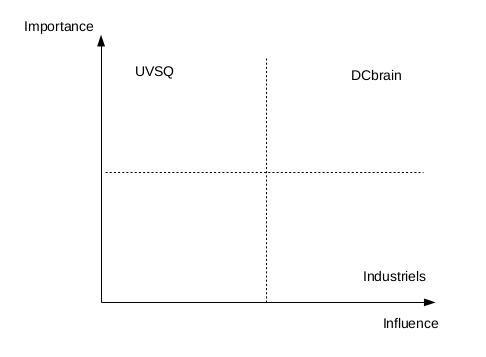
\includegraphics[scale=0.35]{../Cahier/diagPP.png}\end{center}
		\pause \vspace{-0.5em}
		\textbf{Utilisateurs :} membres de DCbrain + industriels du domaine
	\end{frame}	
	
	\section{Contraintes}
	\begin{frame}
		3 exigences contraignantes pour le produit :
		\pause
		\begin{itemize}
			\item Fournir une application web \textbf{\textit{applet}}
			\pause
			\item Développé avec un langage permettant une analyse de données
			\pause
			\item Fournir API d'analyse de données en sortie
		\end{itemize}
		~\\
		\pause
		\textbf{Environnement de fonctionnement :} celui d'une \textbf{\textit{applet}}
			\begin{center}\begin{tikzpicture}[scale=0.5]\begin{scope}[xscale=2,yscale=1.5]	
				\node (USR) at (-3,0) [rectangle,draw] {\begin{tabular}{c}{\tiny Utilisateur}\end{tabular}};
				\node (NAV) at (0,0) [rectangle,draw,fill=blue!25] {\begin{tabular}{c}{\tiny Navigateur web}\end{tabular}};
				\node (APP) at (3,0) [rectangle,draw] {\begin{tabular}{c}{\tiny Application}\end{tabular}};
				\path[->,>=stealth'] (USR) edge[bend left=17] node[anchor=south,above]{{\tiny Accès à l'hôte}} (NAV);
				\path[->,>=stealth'] (NAV) edge[bend left=17] node[anchor=south,above]{{\tiny Intégration de l'application}} (APP);
			\end{scope}\end{tikzpicture}\end{center}
		~\\
		\pause
		\textbf{Applications partenaires :} outils de DCbrain (intégration API)
		\\~\\
		\pause
		\textbf{Temps et budget :} rendu avant le 26/05/2017, aucun budget.
	\end{frame}
	
	\section{Exigences fonctionnelles}
	\begin{frame}
		Sonny
	\end{frame}
	
	\section{Exigences fonctionnelles}
	\begin{frame}
		\begin{center}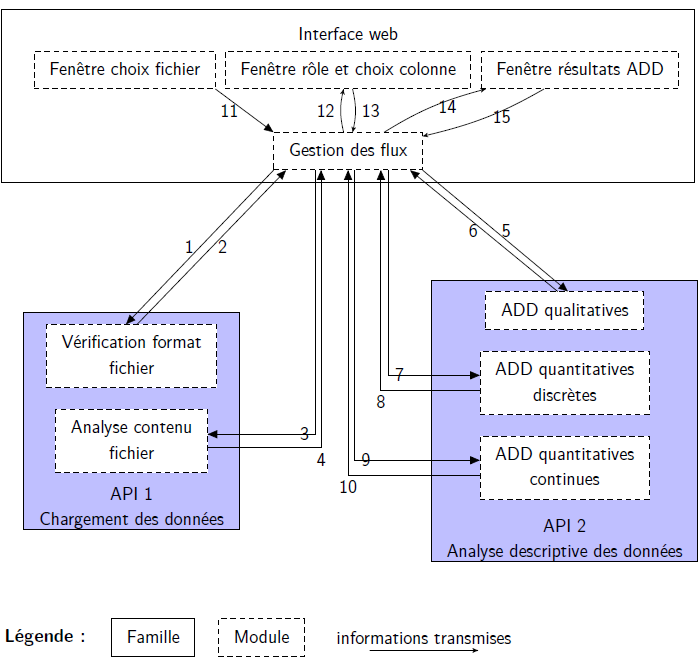
\includegraphics[scale=0.43]{org.png}\end{center}
	\end{frame}
	
	\section{Exigences non fonctionnelles}
	\begin{frame}
		\textbf{Interface utilisateur:} Interface simple, agréable, intuitive et interactive en anglais.\\~\\ 
		\pause
		\textbf{Utilisabilité:} Simple d'utilisation et facile à comprendre.\\~\\
		\pause
		\textbf{Performance:} Réponse fluide et affichage des résultats de l'ordre de la minute.\\~\\
		\pause
		\textbf{Précision et exactitude:} Calculs très précis pour la Moyenne et la Variance. Les autres valeurs seront moins précis.\\~\\
		\pause
		\textbf{Maintenabilité:} Doit pouvoir être maintenu par ses utilisateurs finaux ou par des développeurs. Permettre l'insertion d'éventuels API supplémentaires.\\~\\
		\pause
		\textbf{Sécurité:} Accès à partir d'un navigateur web. Manipulation des données fiables. Pas de manipulation de données à caractère personnel.\\
	\end{frame}
	
	\section{Autres aspects}
	\begin{frame}
		\begin{itemize}
		\item \textbf{Question ouverte} sur l'esthétisme et présentation des résultats.\\~\\
		\pause
		\item \textbf{Choix du langage} : \textbf{Python} compatible avec les applications web et pour les calculs scientifique. \\
		\textbf{HTML} et \textbf{CSS}: Présentation et mise en formes des pages.\\~\\
		\pause
		\item \textbf{Tâche à faire}: Spécifications, Développement de l'application et Compte-rendu.\\~\\
		\pause
		\item \textbf{Contrôle de la finalisation} :Test Unitaires, de validation et acceptation.\\~\\
		\pause
		\item \textbf{Estimation des coûts} de 565 lignes de code.\\~\\
		\pause
		\item \textbf{Répartition des tâches}: Tableau sur la répartition des tâches.\\~\\
		\pause
		\item \textbf{Documentation utilisateur} fournie.\\~\\
		
		
		\end{itemize}
	\end{frame}
	
	\section{Conclusion}
	\begin{frame}
		Deux langages potentiels Java et Python. Notre choix s'est finalisé sur Python.
		\begin{itemize}
		\pause
		\item \textbf{Python} : Langage préconisé par les startups pour construire des applications. 
		\pause
		\item \textbf{Java} : Utilisé par les entreprises ayant les moyens pour le développement et la maintenance du système.
		\end{itemize}
		\pause
		\textbf{Difficultés rencontrées :}  Apprendre une nouvelle démarche et pratique dans un projet à grande ampleur.\\
	\end{frame}	
	
	\section{Bibliographie/sitographie ADD}
	\begin{frame}
	\begin{itemize}
		\item http://www.math.univ-toulouse.fr/~baccini/zpedago/asde.pdf
		\item http://www.math.univ-toulouse.fr/~besse/Wikistat/pdf/st-l-des-uni.pdf
		\item http://iml.univ-mrs.fr/~reboul/cours2.pdf
		\item https://hal.archives-ouvertes.fr/halshs-00287751/document
		\item Wikipédia : Données aberrantes
		\item Exploration de données et méthodes statistiques - Ellipses - Lise Bellanger, Richard Tomassone
		\item Statistique théorique et appliquée: 1. Statistique descriptive et base de l'inférence statistique - 3e édition - de boeck - Pierre Dagnélie
	\end{itemize}
		
	\end{frame}
	
\end{document}
